\subchapter{Creating a new virtual netdev}
{Objective: learn how to interact with net devices in the kernel, and use netlink}

\section{Goals}
 
 \begin{itemize}
 \item Create a very basic driver for a new Layer 2 network protocol
 \end{itemize}
 
\section{Transmit path}

Our driver will behave somewhat like what a 802.1Q driver would, that is we will
receive a frame to be send (in the form of a \kstruct{sk_buff} passed a parameter to
our \code{.ndo_start_xmit} function), containing a fully-formed Ethernet frame :

\begin{center}
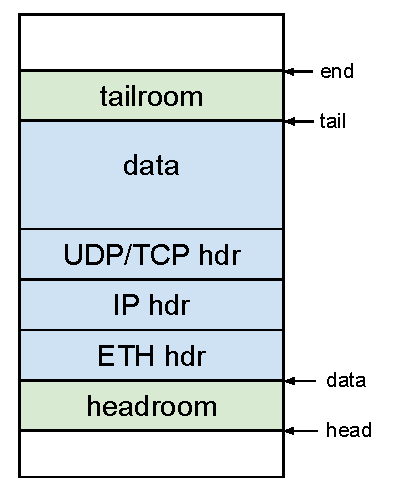
\includegraphics[width=0.3\textwidth]{labs/networking-skb/01_blan_skb.pdf}
\end{center}

Our custom tag needs to be inserted \textbf{before} the Ethernet header, that is, between the Layer 3 header and the Layer 2 header. We therefore need to move the Ethernet header down into the headroom of the SKB.

To guarantee that we have enough space in the headroom, we can add a constraint to our \kstruct{net_device} to indicate
that when \code{skb} are allocated with our device as a destination, there needs to be mode headroom for our tag.

This can be done by setting \code{dev->needed_headroom} to the size of our header, in our \code{bootlinlan_setup} function.

The kernel doesn't provide any helper to move the ethernet header around, so let's re-build our skb header in 3 steps :
\begin{enumerate}
	\item Save a copy fof the original ethernet header, and remove it
	\item Insert our custom tag
	\item Re-add the original ethernet header
\end{enumerate}

\subsection{Consume and copy the original ethernet header}

In the \code{.ndo_start_xmit} callback of our driver, \code{skb->data} points at
the beginning of the ethernet header. You can represent such a header by using \kstruct{ethhdr} objects, which has the size \ksym{ETH_HLEN} (14 bytes).

Copy the \ksym{ETH_HLEN} bytes of \code{skb->data} into such an object.

Then, consume the first \ksym{ETH_HLEN} bytes of the payload section by calling the appropriate \code{skb}-manipulation helper.

\begin{center}
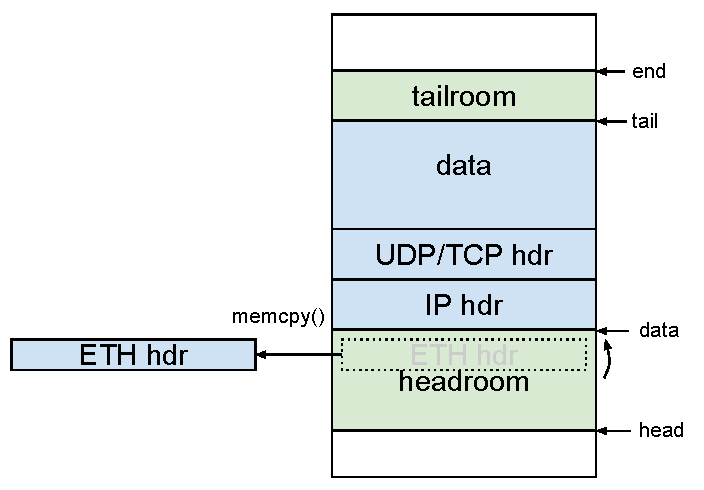
\includegraphics[width=0.6\textwidth]{labs/networking-skb/02_blan_skb.pdf}
\end{center}

\subsection{Re-create the Layer 2 header}

We now need to reconstruct the Layer 2 header. Using the approprate \code{skb} helper, re-increase the size of the \code{skb} by growing into the headroom the size of our blan header.

The helper will return a pointer to the newly grown section, you can directly assign it to your \code{struct blan_hdr}.

Fill-in the \code{blan_hdr} :
\begin{itemize}
	\item The \code{blan->etype} should be the original ethernet header's Ethertype
	\item The \code{blan->id} should be the id associated to our netdev's priv data structure
\end{itemize}

You can now re-construct the Ethernet header. A useful helper for that is \kfunc{eth_header}, which does all the necessary \code{skb} manipulation (looking at its code may give you some clues :) ).

\begin{center}
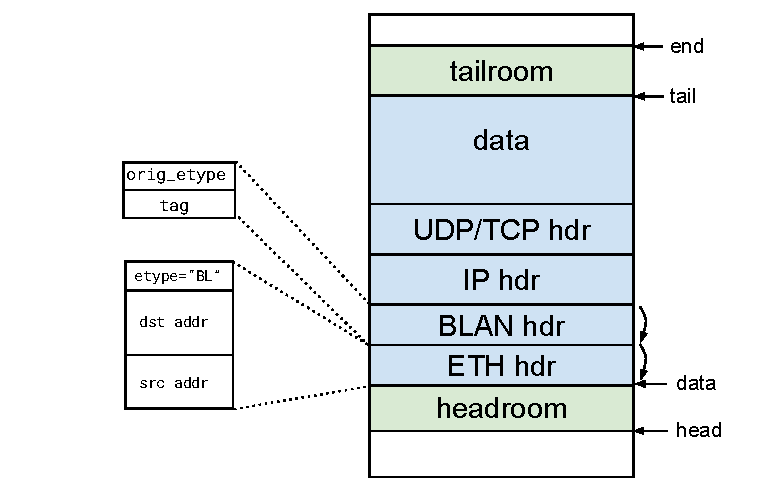
\includegraphics[width=0.6\textwidth]{labs/networking-skb/03_blan_skb.pdf}
\end{center}

Congratulations, it's now time to give your code a test :) Load the module, create the interface and assign it an IP address :

\begin{targetbashinput}
insmod blan.ko
ip link add link lan0 name blan10 type blan
ip address add 192.168.10.2/24 dev blan10
\end{targetbashinput}

Launch \code{tcpdump} on your host machine, on the interface connected to your target :

\begin{hostbashinput}
tcpdump -n -e -i eth0
\end{hostbashinput}

Start a \code{ping} from the target. It will not fully work yet, as we didn't implement the receive path, and the host machine can't understand our protocol :

\begin{targetbashinput}
ping 192.168.10.1
\end{targetbashinput}

